\documentclass{article}
\usepackage[utf8]{inputenc}
\usepackage[english]{babel}
\usepackage [autostyle, english = american]{csquotes}
\MakeOuterQuote{"}
\usepackage{graphicx}
\usepackage{enumerate}
\usepackage{float}
\graphicspath{ {} }
\usepackage{mathtools}
\usepackage{amsmath, amsthm, amssymb, amsfonts}
\usepackage{caption}
\usepackage{bm}
\usepackage{fancyhdr}
\pagestyle{fancy}
\fancyhf{}
\rhead{Ty Darnell}
\lhead{667 Homework 6}

% For derivatives
\newcommand{\deriv}[1]{\frac{\mathrm{d}}{\mathrm{d}x} (#1)}

% For partial derivatives
\newcommand{\pderiv}[2]{\frac{\partial #1}{\partial #2}}

% Integral dx
\newcommand{\dx}{\mathrm{d}x}
\newcommand{\cd}{\overset{d}{\to}}
\newcommand{\cp}{\overset{p}{\to}}
\newcommand{\B}{\beta}
\newcommand{\e}{\epsilon}
\newcommand{\limn}{\lim_{n\to \infty}}
\newcommand{\lm}{\lambda}
\newcommand{\sg}{\sigma}
\newcommand{\hb}{\hat{\beta}}
\newcommand{\sumn}{\sum_{i=1}^{n}}
\newcommand{\hth}{\hat{\theta}}
\newcommand{\lra}{\Leftrightarrow}
\newcommand{\prodn}{\prod_{i=1}^{n}}
\newcommand{\dll}[1]{\dfrac{\partial\ell}{\partial{#1}}}
\newcommand{\mle}{\hat{\theta}_{MLE}}
\newcommand{\mm}{\hat{\theta}_{MM}}
\newcommand{\sumx}{\sum_{i=1}^{n}x_i}
\newcommand{\ta}{\theta}
\newcommand{\qe}{ \ ?\ }
\newcommand{\dt}{\pderiv{}{\ta}}
\newcommand{\lt}[1]{\log(f(#1|\ta))}
\newcommand{\lx}{\lambda(x)}
\newcommand{\samp}{X_1,\dots,X_n \sim}
\newcommand{\te}{\theta_1}
\newcommand{\xm}{x_{(1)}}
\newcommand{\sn}{(\sg^2)}
\newcommand{\pow}{\B(\ta)}
\newcommand{\hyp}[2]{H_0: #1 \text{ vs } H_1: #2}
\newcommand{\pois}[2]{\dfrac{e^{-#1}{#1}^{#2}}{{#2}!}}
\newcommand{\mlr}{\dfrac{f(x|\ta_2)}{f(x|\ta_1)}}
\newcommand{\al}{\alpha}
\newcommand{\bx}{\bar{x}}
\allowdisplaybreaks
\begin{document}
\begin{flushleft}

\section*{Problem 1}
\begin{enumerate}[(a)]
\item

\begin{multline*}\\
i=1 \text{ Placebo} \quad i=2 \text{ Active Treatment}\\
\mu_1=\left[
\begin{array}{rrrrr}
235.93 & 243.17 & 244.76 & 257.60 & 257.48 \\ 
\end{array}
\right]^T\\
\mu_2=\left[
\begin{array}{rrrrr}
226.02 & 245.53 & 252.02 & 256.80 & 254.55 \\ 
\end{array}
\right]^T\\
\Sigma_1=\left[
\begin{array}{rrrrr}
3080.44 & 2342.72 & 2158.73 & 2404.83 & 2086.78 \\ 
2342.72 & 2755.49 & 2261.28 & 2392.10 & 2123.54 \\ 
2158.73 & 2261.28 & 2267.72 & 2184.92 & 1828.96 \\ 
2404.83 & 2392.10 & 2184.92 & 2666.96 & 2012.98 \\ 
2086.78 & 2123.54 & 1828.96 & 2012.98 & 2439.19 \\ 
\end{array}
\right]\\
\Sigma_2=\left[
\begin{array}{rrrrr}
1962.46 & 1302.20 & 1150.85 & 952.35 & 1009.28 \\ 
1302.20 & 1715.22 & 1109.22 & 1023.43 & 1199.37 \\ 
1150.85 & 1109.22 & 1553.90 & 696.86 & 1265.57 \\ 
952.35 & 1023.43 & 696.86 & 1147.61 & 866.61 \\ 
1009.28 & 1199.37 & 1265.57 & 866.61 & 2545.69 \\ 
\end{array}
\right]\\
\textbf{Means over time}\\
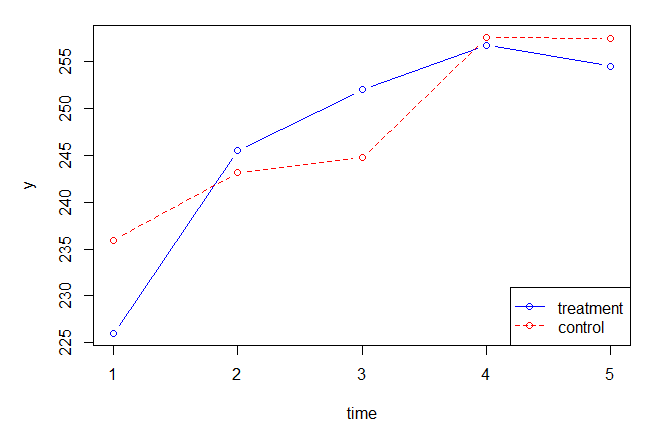
\includegraphics[scale=.5]{meanplot1.png}\\
\end{multline*}
\item
\begin{multline*}\\
\text{Imposing the estamability restrictions and fitting the general two-way anova model}\\
\text{For } j=(2,3,4,5) \text{ we have:}\\
E[Y_{ij}]=\mu+\alpha_2I(group2)+\B_iI{time j}+\gamma_{2j}I(group=2)I(time=j)\\
\left[\begin{array}{r|rrrrr}
\hline
\text{Month} &  0 & 6 & 12 & 20 &24\\
 \hline
P & \mu &\mu+\B_2 & \mu+\B_3& \mu+\B_4 &\mu+\B_5\\
\hline
A & \mu+ \alpha_2 &\mu+\alpha_2+\B_2+\gamma_{22} & \mu+\alpha_2+\B_3+\gamma_{23}& \mu+\alpha_2+\B_4+\gamma_{24} &\mu+\alpha_2+\B_5+\gamma_{25}\\
\hline
\end{array}\right]\\
\text{Treatment effect }=\boldsymbol{\delta}=(\gamma_{22},\gamma_{23},\gamma_{24},\gamma_{25})^T\\
\boldsymbol{\delta} \text{ represents the treament effect on the changes in mean cholesterol level over time}\\
\left[\begin{array}{c|c}
\hat{\delta}&\hat{se}\\
\hline
\gamma_{22}=12.272& 6.194\\
\gamma_{23}=16.418& 6.752\\
\gamma_{24}=4.977& 7.011\\
\gamma_{24}=6.903& 9.887\\
\end{array}\right]\\
\end{multline*}
\item
Wald Chi-square test\\
$H_0:\delta=0$\\
$H_1:\delta\neq 0$\\
Wald $\chi^2=7.86$ df=4\\
p-value$=.0968>.05$ Thus fail to reject $H_0$\\
Not enough evidence to suggest $\delta$ is not equal to 0. The mean response profiles are statistically the same for the two groups.
\item
\begin{multline*}
\left[\begin{array}{r|rrrrr}
\hline
\text{Month} &  0 & 6 & 12 & 20 &24\\
\hline
P & \mu &\mu+\B_2 & \mu+\B_3& \mu+\B_4 &\mu+\B_5\\
\hline
A & \mu &\mu+\B_2+\gamma_{22} & \mu+\B_3+\gamma_{23}& \mu+\B_4+\gamma_{24} &\mu+\B_5+\gamma_{25}\\
\hline
\end{array}\right]\\
\text{Treatment effect }=\boldsymbol{\delta}=(\gamma_{22},\gamma_{23},\gamma_{24},\gamma_{25})^T\\
\boldsymbol{\delta} \text{ represents the treament effect on the changes in mean cholesterol level over time}\\
\left[\begin{array}{c|c}
\hat{\delta}&\hat{se}\\
\hline
\gamma_{22}=9.478& 5.596\\
\gamma_{23}=12.886& 5.85\\
\gamma_{24}=1.614& 6.208\\
\gamma_{24}=3.003& 9.064\\
\end{array}\right]\\
\end{multline*}

\item
\begin{multline*}\\
\text{t}=time \quad x=I(group2)\\
\text{group 1: } E(Y_{ij})=\B_1+\B_2*t_{ij}+\B_3*t_{ij}^2\\
\text{group 2: } E(Y_{kj})=\alpha_1+\alpha_2*t_{kj}+\alpha_3*t_{kj}^2\\
\text{Restrictions: } E(Y_i1)=E(Y_{k1}), \quad \B_1=\alpha_1\\
\left[\begin{array}{l|lllll}
	\hline
	\text{Month} &  0 & 6 & 12 & 20 &24\\
	\hline
	P & \mu &\mu+6t+36t^2 & \mu+12t+144t^2& \mu+20t+400t^2 &\mu+24t+576t^2\\
	\hline
	A & \mu &\mu+6t+36t^2 & \mu+12t+144t^2+& \mu+20t+400t^2+ &\mu+24t+576t^2+\\
	& & +6xt+36xt^2 &+12xt+144xt^2 &20xt+400xt^2&24xt+576xt^2\\
	\hline
	\end{array}\right]\\
	\text{Treatment effect }=\boldsymbol{\delta}=(xt,xt^2)^T\\
	\boldsymbol{\delta} \text{ represents the treament effect on the changes in mean cholesterol level over time}\\
	\left[\begin{array}{c|c}
	\hat{\delta}&\hat{se}\\
	\hline
	xt=1.937 & .823\\
	xt^2=-.086 & .037\\
	\end{array}\right]\\
	\end{multline*}
	Wald Chi-square test\\
	$H_0:\delta=0$\\
	$H_1:\delta\neq 0$\\
	Wald $\chi^2=5.89$ df=2\\
	p-value$=.0527>.05$ Thus fail to reject $H_0$\\
	Not enough evidence to suggest $\delta$ is not equal to 0. The mean response profiles are statistically the same for the two groups.\\
	\item
\begin{multline*}\\
\text{Treatment Effect on the changes in mean cholesterol level over time }=\lambda=(\alpha_2,\gamma_{23},\gamma_{24},\gamma_{25})\\
\left[\begin{array}{c|c}
\hat{\lambda}&\hat{se}\\
\hline
\alpha_2=12.272 &6.194\\
\gamma_{23}=4.028&5.979\\
\gamma_{24}=-8.07&6.097\\
\gamma_{25}=-5.226&8.901\\
\end{array}\right]\\
\end{multline*}
\item
	Wald Chi-square test\\
$H_0:\lambda=0$\\
$H_1:\lambda \neq 0$\\
Wald $\chi^2=7.99$ df=4\\
p-value$=.0919>.05$ Thus fail to reject $H_0$\\
Not enough evidence to suggest $\lambda$ is not equal to 0. The mean response profiles are statistically the same for the two groups.\\
\item
\begin{multline*}\\
\text{Treatment Effect on the changes in mean cholesterol level over time }=\lambda^*=(\alpha_2,\gamma_{23},\gamma_{24},\gamma_{25})\\
\left[\begin{array}{c|c}
\hat{\lambda^*}&\hat{se}\\
\hline
\alpha_2=9.023 & 5.653\\
\gamma_{23}=4.144& 5.937\\
\gamma_{24}=-7.394&6.03\\
\gamma_{25}=-5.218&8.842\\
\end{array}\right]\\
\end{multline*}
\item
	Wald Chi-square test\\
$H_0:\lambda^*=0$\\
$H_1:\lambda^* \neq 0$\\
Wald $\chi^2=6.54$ df=4\\
p-value$=.1623>.05$ Thus fail to reject $H_0$\\
Not enough evidence to suggest $\lambda^*$ is not equal to 0. The mean response profiles are statistically the same for the two groups.\\
\item
Full LRT test\\
$H_0:\lambda^*=0$\\
$H_1:\lambda^* \neq 0$\\
$-2Log(L)_{Full}=3218.6$ df=8\\
$-2Log(L)_{Reduced}=3225.1$ df=4\\
$\chi^2=3225.1-3218.6=6.5$ df=4\\
p-value$=.165>.05$ Thus fail to reject $H_0$\\
Not enough evidence to suggest $\lambda^*$ is not equal to 0. The mean response profiles are statistically the same for the two groups.\\
\item
You need the following assumptions to guarantee $\lambda=\lambda^*$:\\
1) No interaction\\
2) At baseline the two groups have the same mean
\end{enumerate}
\end{flushleft}
\end{document}
